\subsection{Flip-Flop D}

O flip-flop D (Data) é o mais utilizado em sistemas digitais reais devido à sua simplicidade. Ele possui apenas uma entrada:

\begin{itemize}
    \item $D$: Data
\end{itemize}

\begin{center}
\begin{tabular}{c | c}
D & $Q_{t+1}$ \\
\hline
 0 & 0 \\
 1 & 1 \\
\end{tabular}
\end{center}

Ou seja, em $t+1$ o circúito assume o estado D.

\begin{figure}[H]
    \centering
    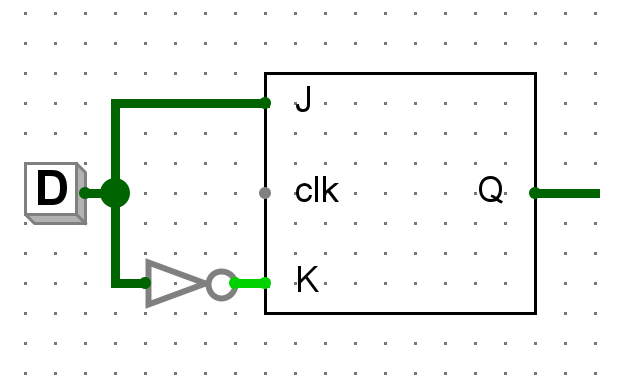
\includegraphics[width=0.5\linewidth]{images/D-FF.png}
    \caption{Implementação do Flip Flop tipo D a partir do Flip Flop JK}
    \label{fig:D-FF}
\end{figure}

Apesar de ser possível fazer esta implementação no Minecraft,

\begin{figure}[H]
    \centering
    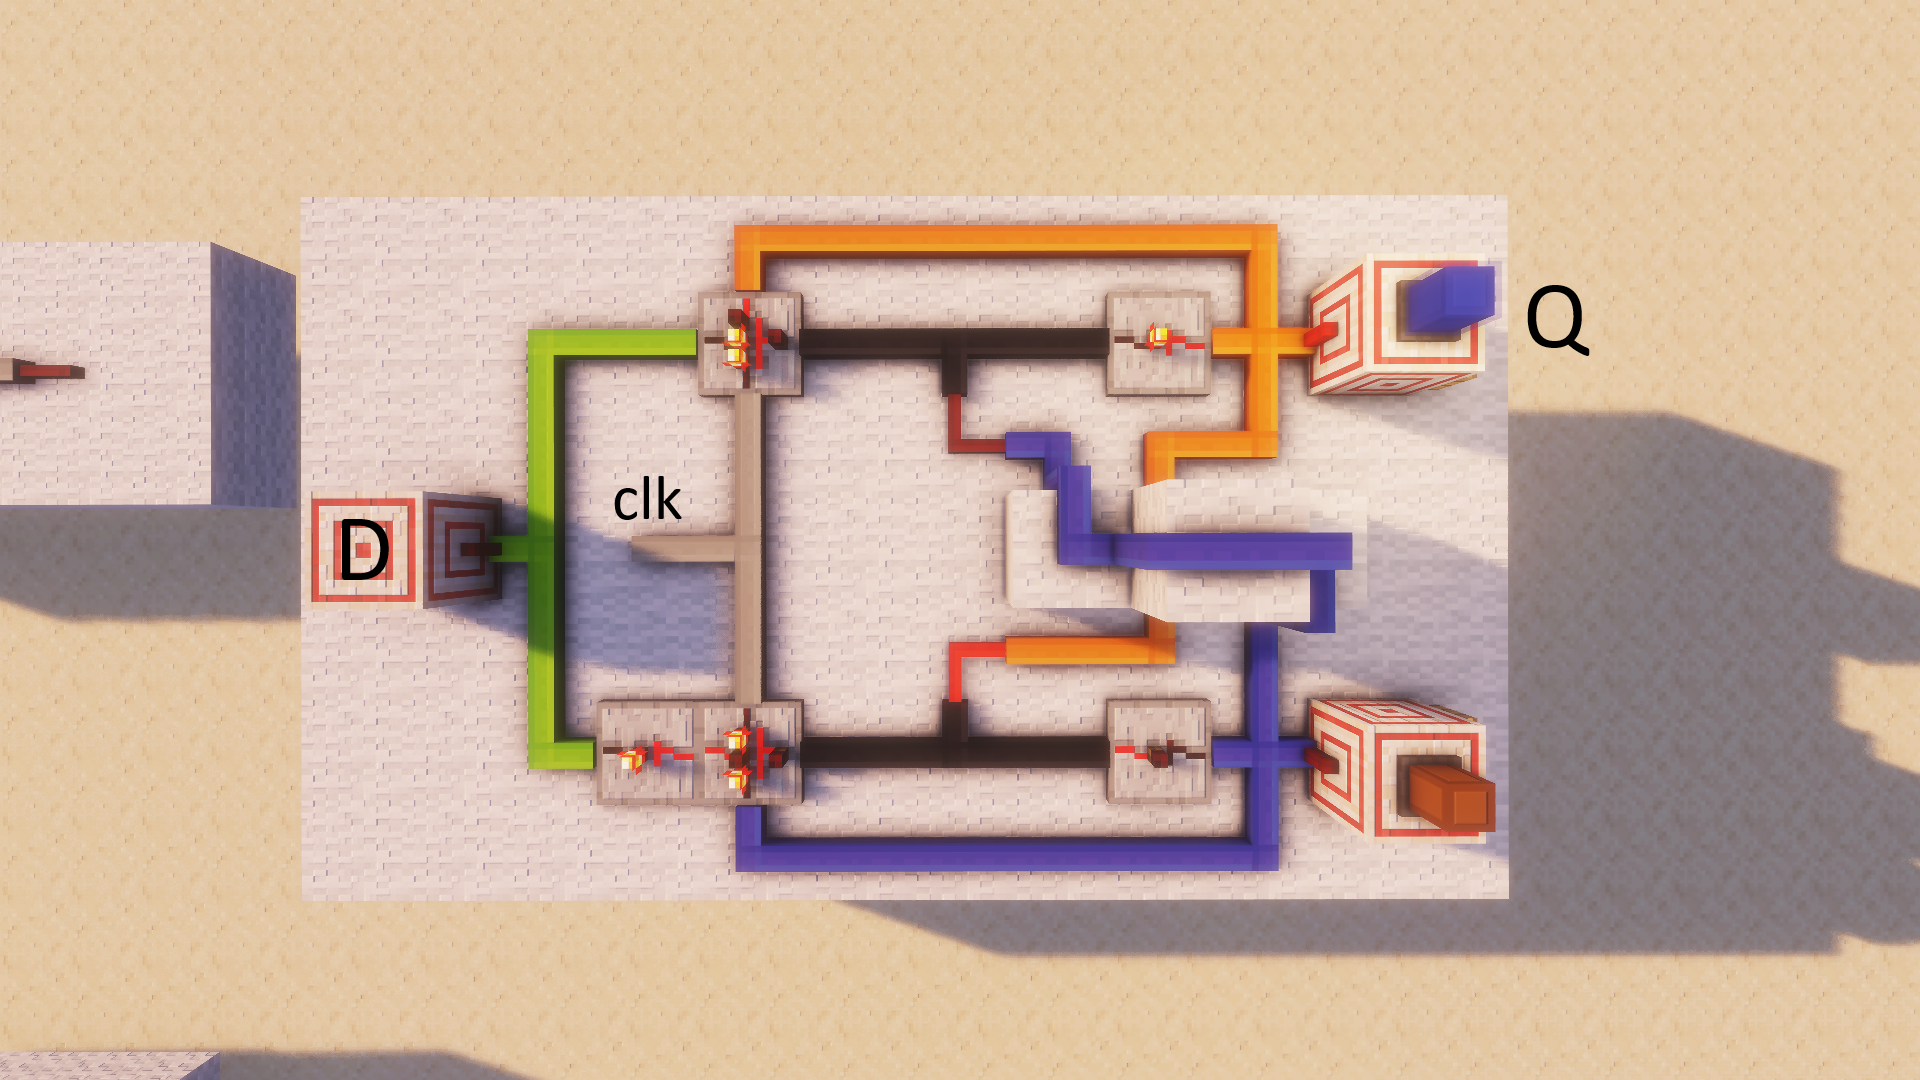
\includegraphics[width=0.8\linewidth]{images/D-FF-redstone-expanded.png}
    \caption{Implementação do Flip Flop tipo D a partir do Flip Flop JK em redstone}
    \label{fig:D-FF-redstone-expanded}
\end{figure}

tipicamente, aproveita-se da propiedade de trava dos repetidores de redstone para implementar o Flip Flop tipo D, na seguinte disposição:

\begin{figure}[H]
    \centering
    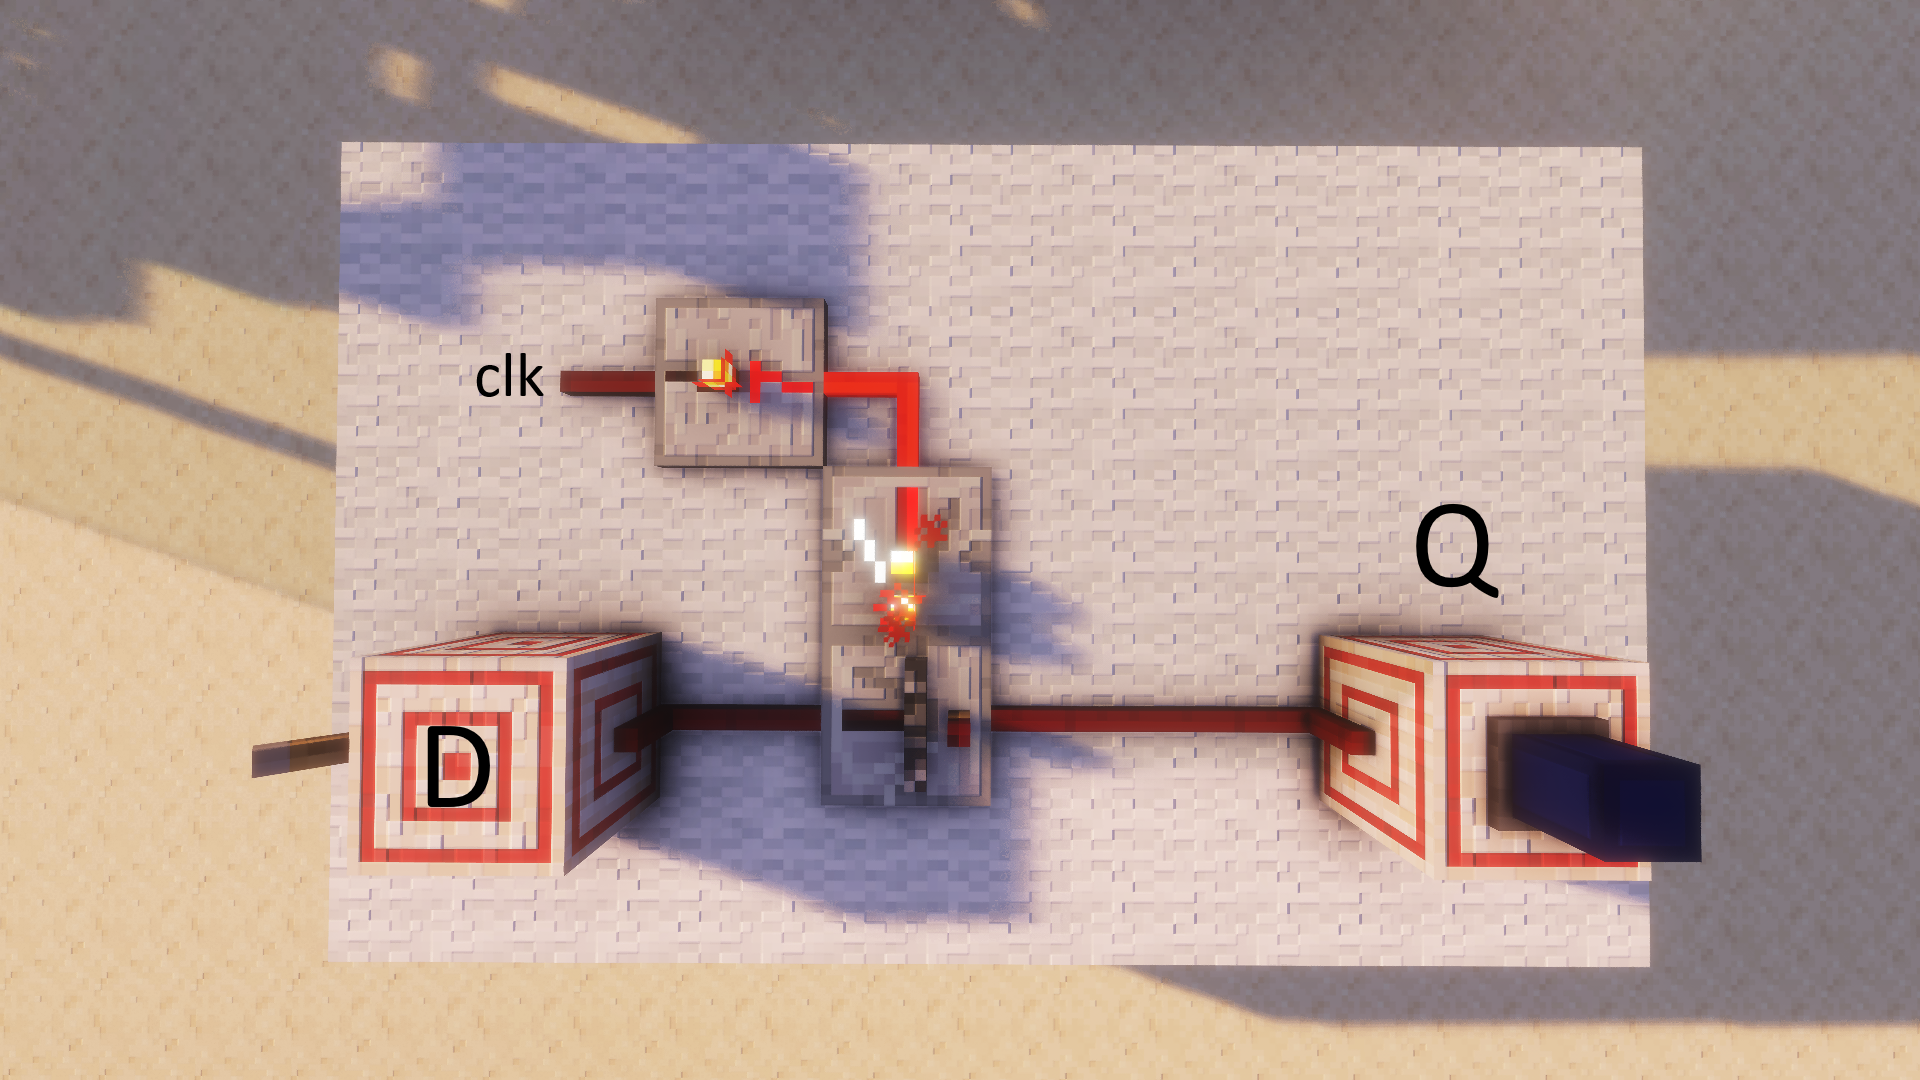
\includegraphics[width=0.8\linewidth]{images/D-FF-redstone.png}
    \caption{Implementação do Flip Flop tipo D a partir de repetidores de redstone}
    \label{fig:D-FF-redstone}
\end{figure}

De forma simplificada, enquanto $clk=0$ o repetidor trava no estado $Q$, quando o sinal de clock sobe, o repetidor é destravado e o estado de D é liberado para passar por ele. Assim, quando o clock desce, o repetidor trava no estado de $D$.

Entretanto, existe um atraso entre o clock e o lock efetivo do sistema. Observe o diagrama temporal desse sistema. No exemplo considerado, o clock possui período de $10$ Game Ticks e duty cycle de $50\%$. O repetidor está configurado para $1$ RT, e o portão NOT introduz um atraso de $1$ GT.

\begin{figure}[H]
    \centering
    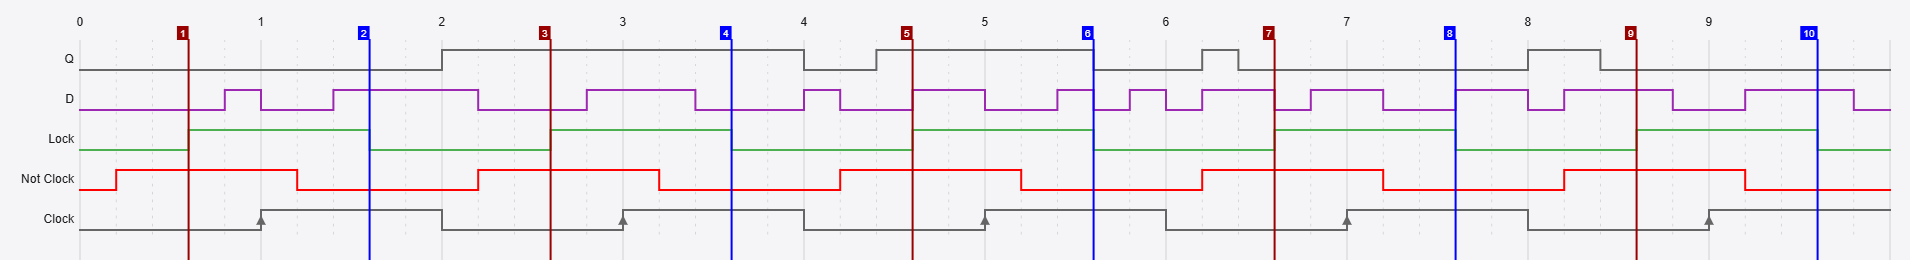
\includegraphics[width=1\linewidth]{images/D-FF-time-diagram-redstone.png}
    \caption{Diagrama temporal do flip flpo tipo D descrito}
    \label{fig:D-FF-time-diagram-redstone}
\end{figure}

O instante efetivo de captura do valor de $D$ ocorre imediatamente antes do travamento do circuito. Considerando o atraso total até o bloqueio ($t_{lock}$) e o atraso interno do repetidor ($t_{rep}$), o valor armazenado corresponde ao sinal de entrada no instante:

\begin{align*}
t &= t_{lock} - t_{rep}
\end{align*}

O instante de travamento pode ser expresso em função do clock como:

\begin{align*}
t_{lock} &= ( t_{descida}) + t_{delay} \\
&=( t_{subida} + T \cdot \text{duty cycle}) + t_{delay}
\end{align*}

Portanto, 

\begin{align*}
t &= ( t_{descida}) + t_{delay} - t_{rep} \\
&= ( t_{subida} + T \cdot \text{duty cycle}) + t_{delay} - t_{rep}
\end{align*}

onde $t_{delay}$ representa o atraso acumulado dos componentes do circuito. 

Substituindo, as variáveis para este exemplo, obtemos:

\begin{align*}
t &= t_{descida} + 1 \\
&= t_{subida} + 6
\end{align*}

Observa-se, portanto, que o instante de amostragem não coincide exatamente com a borda do clock, sendo deslocado pelos atrasos de propagação do circuito.